% Author: Marek Fiser <tikz at marekfiser.cz>
% MESIF protocol: http://en.wikipedia.org/wiki/MESIF_protocol
%Template found online and modified to fit specific needs
\documentclass[tikz, border=10pt]{standalone}
\usetikzlibrary{arrows}
\usetikzlibrary{positioning}
\begin{document}
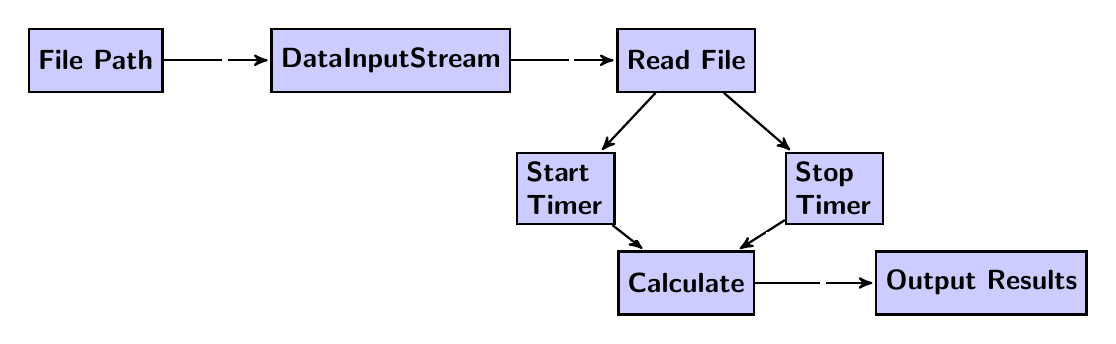
\begin{tikzpicture}[->,>=stealth',shorten >=1pt,auto,node distance=3.75cm,
  thick,main node/.style={rectangle,fill=blue!20,draw,
  font=\sffamily\bfseries,minimum size=8mm}]

  \node[main node] (R) {Read File};
  \node[main node] (DIS) [left of=R] {DataInputStream};
  \node[main node] (IN) [left of=DIS] {File Path};
  \node[main node] (STR) [text width=1cm, below left=.75cm and .01cm of R] {Start Timer};
  \node[main node] (STP) [text width=1cm, right=2.15cm of STR] {Stop Timer};
  \node[main node] (C) [below=2cm of R] {Calculate};
  \node[main node] (OUT) [right of=C] {Output Results};

  \path[every node/.style={font=\sffamily\small,
  		fill=white,inner sep=1pt}]
  		
  	%Shows file Path passed into Data Input stream %
  	(IN) edge [left=20] node[right=.5mm] {} (DIS)
  	%Shows DIS Reading file
  	(DIS) edge [left=20] node[right=.5mm] {} (R)
  	%Shows Read File Starts Timer When Called
  	(R) edge [left=20] node[right= 1mm] {} (STR)
  	(R) edge [left=20] node[right= 1mm] {} (STP)
  	%Shows Start Timer & Stop Timer Connect with Calculate
    	(STR) edge [left=20] node[right=.5mm] {} (C)
    	(STP) edge [left=20] node[right=.5mm] {} (C)
    	%Shows Stop Timer Outputing Results
  	(C) edge [left=20] node[right=.5mm] {} (OUT);    
	
\end{tikzpicture}
\end{document}\textsl{•}